\chapter{More Advanced \KK Reduction}

In the previous chapter, it was seen that the \KK reduction of a scalar field on a total spacetime, which is a direct product of a $D$-dimensional spacetime and a compact manifold, is done with ease, but the moral of the procedure is that the effective mass is inversely proportional to the typical length, {\it a.k.a.} radius, of the compact manifold.

Therefore, if there is a phenomenological argument to assume that the compact manifold has a typical radius $R\lll \SI{e-2}{\TeV}$, then only the massless modes of the effective theory are worth tho be analysed. Thus, it is necessary to learn how to count the number of massless fields on the lower dimensional theory. The task is achieved by using topological information of the compact manifold.

\section{Massless Fields and Harmonic Forms}

It was shown in the three examples in Sec.~\ref{sec:KKs:s1}, Sec.~\ref{sec:KKs:s2} and Sec.~\ref{sec:KKs:t2}, when the \KK reduction is done on a compact manifold, $\mathcal{K}$, the massless scalar fields come from the number of nonequivalent harmonic forms on $\mathcal{K}$. This number is independent of the geometry of $\mathcal{K}$, which can be heuristically argued from the fact that is independent or $R$, but is a topological quantity, i.e., a topological invariant.

In a previous chapter, the de Rham cohomology group was defined as
\begin{align}
  H^p(M)\equiv \frac{\Ker\(\df:C^\infty\(\Lambda^{p}(M)\)\to C^\infty\(\Lambda^{p+1}(M)\) \)}{\Im\(\df:C^\infty\(\Lambda^{p-1}(M)\)\to C^\infty\(\Lambda^{p}(M)\)\)},
\end{align}
therefore, the number of nonequivalent harmonic $p$-forms equals the dimension of the $p$-th de Rham cohomology group, which is commonly known as the $p$-th Betti number, $b^p(M)$.

From the previous paragraph, the number of massless scalar fields in the lower dimensional effective theory is $b^0(M)$, while the number of massless 1-forms is $b^1(M)$, and so on! 
Nonetheless, the counting is not necessarily right, since the dimensional reduction of $p$-forms on a compact $n$-dimensional manifold yields to all kind of forms from $(p-n)$ to $p$ order.

In the next sections a heuristic way to compute Betti numbers of simple manifold is shown, and the dimensional reduction of a rich theory is considered.


\section{Cohomology and Homology}

The cohomology groups are not intuitive to calculate. However, de Rham showed that there is a duality between the cohomology group and the homology group.


\begin{Thm}\label{thm:dR}
  If $M$ is a compact manifold, $H^r (M)$ and
  $H_r (M)$ are finite dimensional. Moreover the exists a map
  \begin{align}
    \Lambda    : H^r (M) \times H_r (M) \to \R,
  \end{align}
  which is bilinear and non-degenerate. Thus, $H^ r (M)$ is the dual vector space of $H_r (M)$.
\end{Thm}

From Thm. \ref{thm:dR}, it follows that $b^r(M)=\dim(H^r(M)) = \dim(H_r(M))$, and the later is nothing but the number of nonequivalent, un-shrinkable, $r$-cycles (modulus $r$-boundaries) defined on $M$.  These $r$-cycles can be count via the homotopy group, $\pi_r(M):S^r\to M$.


%% \begin{center}
%%   \begin{tikzpicture}
%%     \begin{axis}[
%%           hide axis,
%%           view={40}{40}
%%       ]
      
%%       \addplot3 [
%%         surf, shader=faceted interp,
%%         point meta=x,
%%         colormap/greenyellow,
%%         samples=20,
%%         samples y=40,
%%         %z buffer=sort,
%%         domain=0:180,
%%         y domain=0:360
%%       ] (
%%                 {sin(x)*cos(y)},
%%                 {sin(x)*sin(y)},
%%                 {cos(x)}
%%       );
      
%%     \end{axis}
%%   \end{tikzpicture}
%% \end{center}

Since the formal theory of this topological invariant is far from the scope of this manuscript, only examples are given in which the $r$-cycles are counted, and finally the {\bf K\"unneth formula} for calculating the Betti numbers of Cartesian products of manifolds is stated.

\subsection{Betti Numbers Though Examples}

Concentrate in the $\pi_0(M)$, for an arbitrary manifold $M$. Since $S^0$ is a point, $b_0(M)$ counts the number of nonequivalent points on $M$, i.e., the number of connected components. Thus,
\begin{align}
  b_0(\R^n)=b_0(S^n)=b_0(T^n) &= 1,\\
  b_0(O(N)) &= 2\qquad\text{for }N>1,
\end{align}
in the last line, $O(N)$ is the $N$-th orthogonal group, and the result is 2 because $O(N)$ has two disconnected components: transformations with $\det(M)=1$ and transformations with $\det(M)=-1$.


\begin{center}
  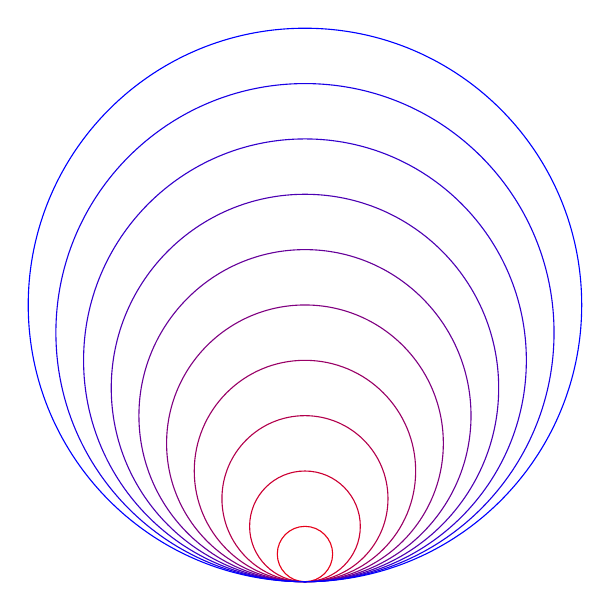
\begin{tikzpicture}
    \foreach \r in {0,10,...,100}
    \draw[color=blue!\r!red] (0,0) arc  (-90:270:\r pt);
  \end{tikzpicture}
\end{center}
